\documentclass[a4paper, 11pt]{article}
\usepackage{amsmath}
\usepackage{graphicx}
\usepackage{geometry}
\usepackage{listings}
\geometry{scale=0.8}

\title{	
\normalfont \normalsize
\textsc{School of Data and Computer Science, Sun Yat-sen University} \\ [25pt] %textsc small capital letters
\rule{\textwidth}{0.5pt} \\[0.4cm] % Thin top horizontal rule
\huge  The Maze Problem\\ % The assignment title
\rule{\textwidth}{2pt} \\[0.5cm] % Thick bottom horizontal rule
\author{Shixuan Lee 15336085}
\date{\normalsize\today}
}


\begin{document}
\maketitle
\newpage
\tableofcontents
\newpage
\section{codes}
\lstset{language=C++}
\lstset{breaklines=true}
\begin{lstlisting}
#include <iostream>
using namespace std;

const int MAX_N = 0x3f3f3f3f;
char maze[5][5];
int dis[5][5];
int dx[4] = {1, 0, -1, 0}, dy[4] = {0, 1, 0, -1};
int top = 0, rear = 1;
struct S{
	int x;int y;
	int pas;	
}que[100];

void print(int i){
	if(que[i].pas != -1){
		print(que[i].pas);
		cout << "(" << que[i].x << "," << que[i].y << ")" << endl;
	}
	
}
void findpath(){
	for(int i = 0; i < 5; i++)
		for(int j = 0; j < 5; j++)
			dis[i][j] = MAX_N;
	dis[0][0] = 0;
	que[0].x = 0;
	que[0].y = 0;
	que[0].pas = -1; 
	while(top < rear){
		int k = 0; 
		for(k; k < 4; k++){
			int nx = que[top].x + dx[k];
			int ny = que[top].y + dy[k];
			if(nx == 4 && ny == 4){
				print(top);
			}
			if(0 <= nx && nx < 5 && 0 <= ny && maze[nx][ny] != '1' && dis[nx][ny] == MAX_N){
				que[rear].x = nx;
				que[rear].y = ny;
				que[rear].pas = top;
				dis[nx][ny] = dis[que[top].x][que[top].y] + 1;
				rear++;
			}
		}
		top++;
	}
}

int main(){
	cout << "Please input the 5x5 maze:" << endl;
	for(int i = 0; i < 5; i++){
		for(int j = 0 ; j < 5; j++){
			cin >> maze[i][j];
		}
	}
	cout << "The result is:" << endl;
	cout << "(0,0)" << endl;
	findpath(); 
	cout << "(4,4)" << endl;
	return 0;
}


\end{lstlisting}
\section{Results}
\centering
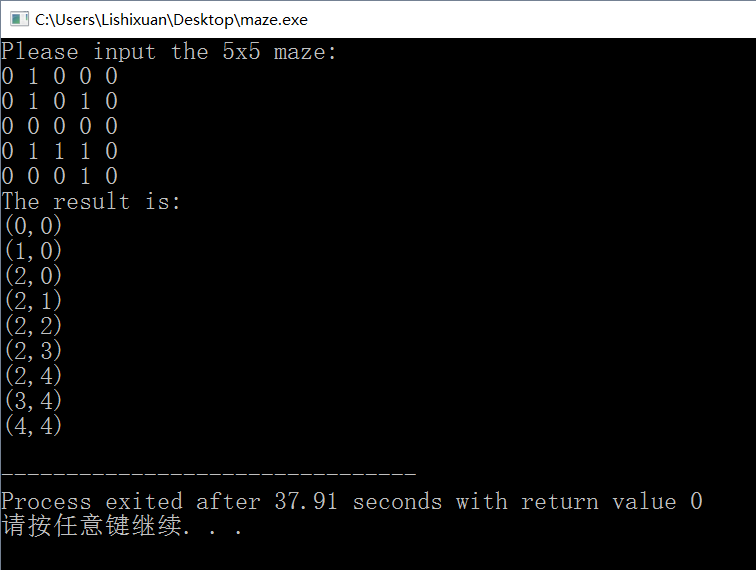
\includegraphics[width=15cm]{Maze.png}
%\tableofcontents
%\newpage

\end{document} 